\documentclass[10pt]{beamer}

\usetheme{moloch}

\usepackage{booktabs}
\usepackage[scale=2]{ccicons}

\usepackage{multirow}
\usepackage{pgfplots}
\usepgfplotslibrary{dateplot}
\usepackage{tikzpeople}
\usepackage{tikz}
\usetikzlibrary{overlay-beamer-styles}
\usetikzlibrary{backgrounds}
\usetikzlibrary{shapes}
\usetikzlibrary{shadings}

\usepackage{svg}
\usepackage{fontawesome5}
\usepackage{amsmath}
\usepackage{amssymb}

\usepackage{algorithm}
\usepackage{float}
\usepackage{algpseudocode}
% to \uncover a \procedureblock
\usepackage{adjustbox}

\algrenewcommand\algorithmicrequire{\textbf{Input:}}
\algrenewcommand\algorithmicensure{\textbf{Output:}}
\newcommand{\kkk}{\mathbf{k}}
\newcommand{\KKK}{\mathbf{K}}
\newcommand{\rrr}{\mathbf{r}}
\newcommand{\iNTT}{$\mathsf{iNTT}$}
\newcommand{\bch}{\mathsf{BCH}}
\newcommand{\intt}{\mathsf{iNTT}}
\newcommand{\leap}{\textsc{Leap}}
\usepackage{xcolor}
\definecolor{mBGcol}{HTML}{fafafa}
\definecolor{colA}{HTML}{990099}
\definecolor{colC}{HTML}{b6b6b6}
\definecolor{colB}{HTML}{00b300}
\definecolor{colD}{HTML}{2eb8b8}
\definecolor{thirdColor}{HTML}{6A5ACD}


\newcommand{\bv}[1]{\mathbf{#1}}
\usepackage[lambda,landau,operators,probability,sets,logic,advantage,complexity,asymptotics,notions,mm,primitives,ff,adversary,advantage]{cryptocode}

\title{OPRFs in the Wild}
\subtitle{A Survey of Real-World Deployments}
\date{7$^{th}$ of March, 2026}
\author{Daniel Escudero, \underline{Lena Heimberger}, Daniel Kales, Christian
Rechberger, Verena Schröppel, Roman Walch}
\institute{RWMPC 2026, Taipei}
\titlegraphic{\vspace{-2em}
\includegraphics[height=1cm]{figures/logo.pdf}\hfill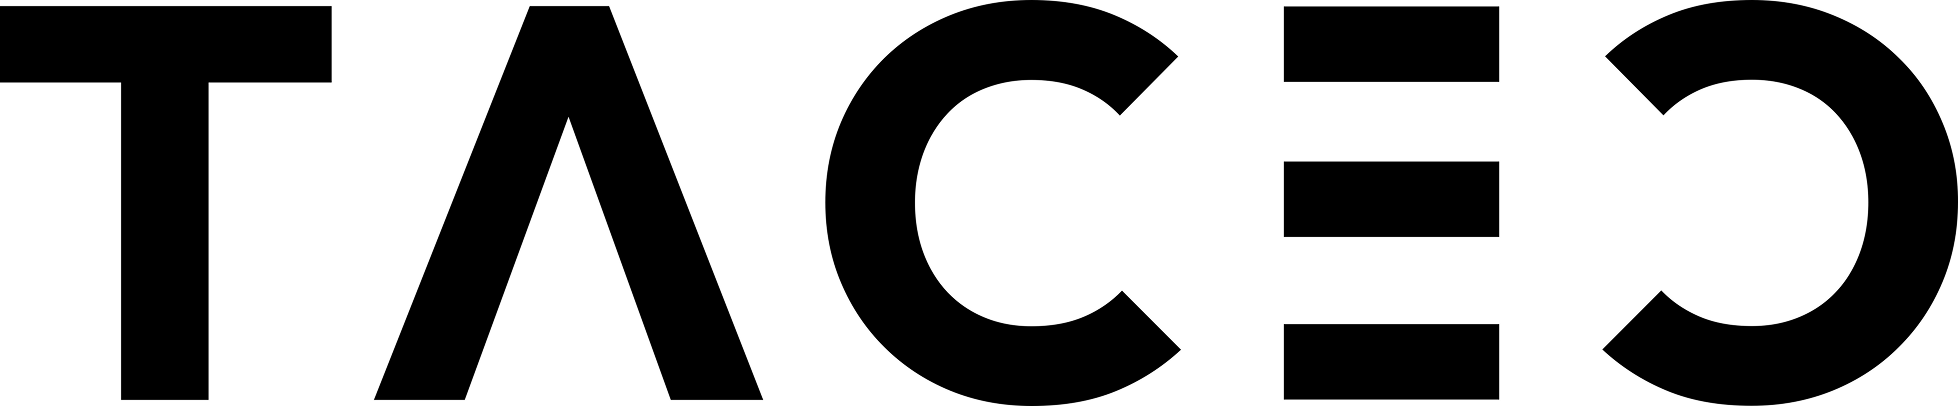
\includegraphics[height=0.8cm]{figures/taceo.png}}
\pgfplotsset{compat=1.18}

\begin{document}

\maketitle

% Brief intro to OPRFs: what they are and why we care
\begin{frame}
  \frametitle{Have you ever wanted to...}
  \begin{itemize}
    \item $\ldots$ send a hash over a wire?\pause
    \item $\ldots$ intersect a set privately?\pause
    \item $\ldots$ generate unlinkable tokens?\pause
    \item $\ldots$ generate MPC-friendly deterministic identifiers?\pause
    \item $\ldots$ take your low-entropy input and get a high-entropy output?
  \end{itemize}

  % TODO put in logos
\end{frame}


% Real-world motivation: Why PSI matters for contact discovery, private databases, threat intelligence sharing
\begin{frame}
  \frametitle{You may want to consider an OPRF!}
  \begin{tikzpicture}[every node/.style={minimum width=1.5cm},scale=0.8]

    \node[alice, monitor, shirt=blue!40!black, minimum size=1.5cm, label=Client] (alice)
      {};
    \node[scale=2.67, label=Server, xshift=3.5cm] (server) {{\large{\faServer}}};
    \node[scale=2.67, label=compute, xshift=1.9cm] (hashfunction) {\({y
      \coloneqq F_k(x)}\)};

    \node(Alicetext) [below of=alice,xshift=1cm, yshift=-0.8cm,text
      width=3cm, text=gray]{input \(x \in \mathcal{X}\), gets \(y\)};
    \node(Servertext) [below of=server, xshift=0.5cm,yshift=-0.5cm,text
      width=3cm,text=gray]{key \(k\in \mathcal{K}\)};
  \end{tikzpicture}
\end{frame}


\begin{frame}
  \frametitle{Pseudorandom Functions \cite{C:GolGolMic84,GolGolMic86} }
  \begin{itemize}
    \item deterministic and polynomial-time function 
    \item hard to distinguish output $y$ from a randomly chosen element from
      $y'\in\mathcal{Y}$.
    \item relatively weak guarantees!
  \end{itemize}\pause
  \bigskip
  \begin{exampleblock}{Simple PRF over elliptic curves}
    Sample $k$ and compute PRF as $y=\mathsf{hash\_to\_curve}(x)*k$\\ Remove algebraic structure with
    $H(y)$
  \end{exampleblock}
\end{frame}

% \begin{frame}
%   \frametitle{Definitions}
%   \centering
%   \begin{exampleblock}{Oblivious Pseudorandom Function}
%     An oblivious pseudorandom function~(OPRF)~\cite{TCC:FIPR05} is a protocol between two parties. One
%     party holds the secret key $k$ and the other holds their secret input $x$.
%     The OPRF privately realizes the joint computation outputting $F_k(x)$ for a PRF $F$ to the
%     party holding $x$, and nothing to the party holding $k$.
%     \label{def:oprf}
%   \end{exampleblock}\pause
%   \alert{
%     Sending a hash over a wire? Use an OPRF instead!
%   }
% 
% \end{frame}

\begin{frame}{Blind-evaluate-unblind: 2HashDH}
  \procedureblock[mode=text]{}{%
    \textbf{Client}\((x)\) \> \> \textbf{Server} \((k)\)\\
    Sample \(r\) \> \sendmessageright*[14em]{b \coloneqq
    \mathsf{hash\_to\_group}(x) * r} \> \\
    \(y=r^{-1}*c\) \> \sendmessageleft*[14em]{{c \coloneqq k * b}}\\
    \(= r^{-1}* k * b \)\\
    \(= \mathsf{hash\_to\_group}(x) * k \)\\
  output $H(y)$ }
\end{frame}

\begin{frame}{What about other constructions? }
  \centering
  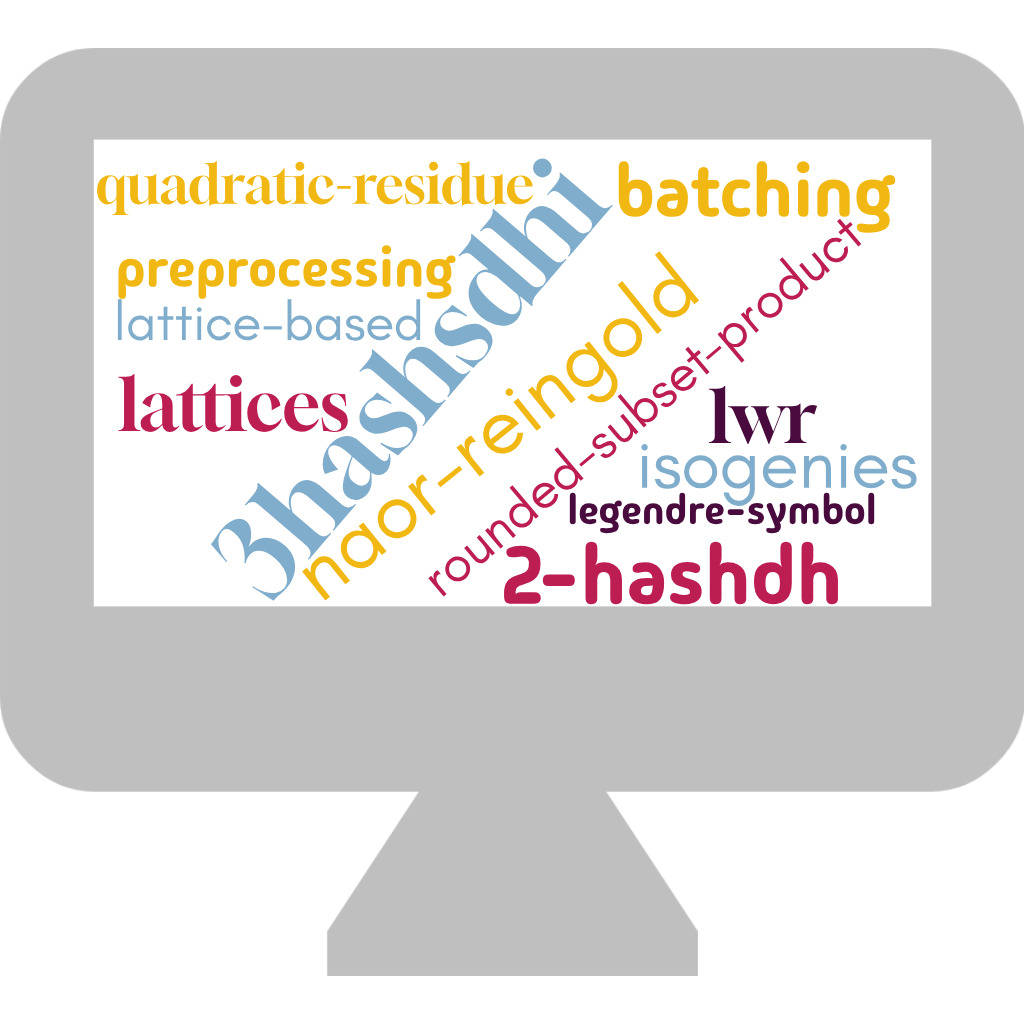
\includegraphics[scale=0.25]{figures/wordcloud-oprfs.jpg}
\end{frame}

\begin{frame}{What about other constructions? }
  \centering
  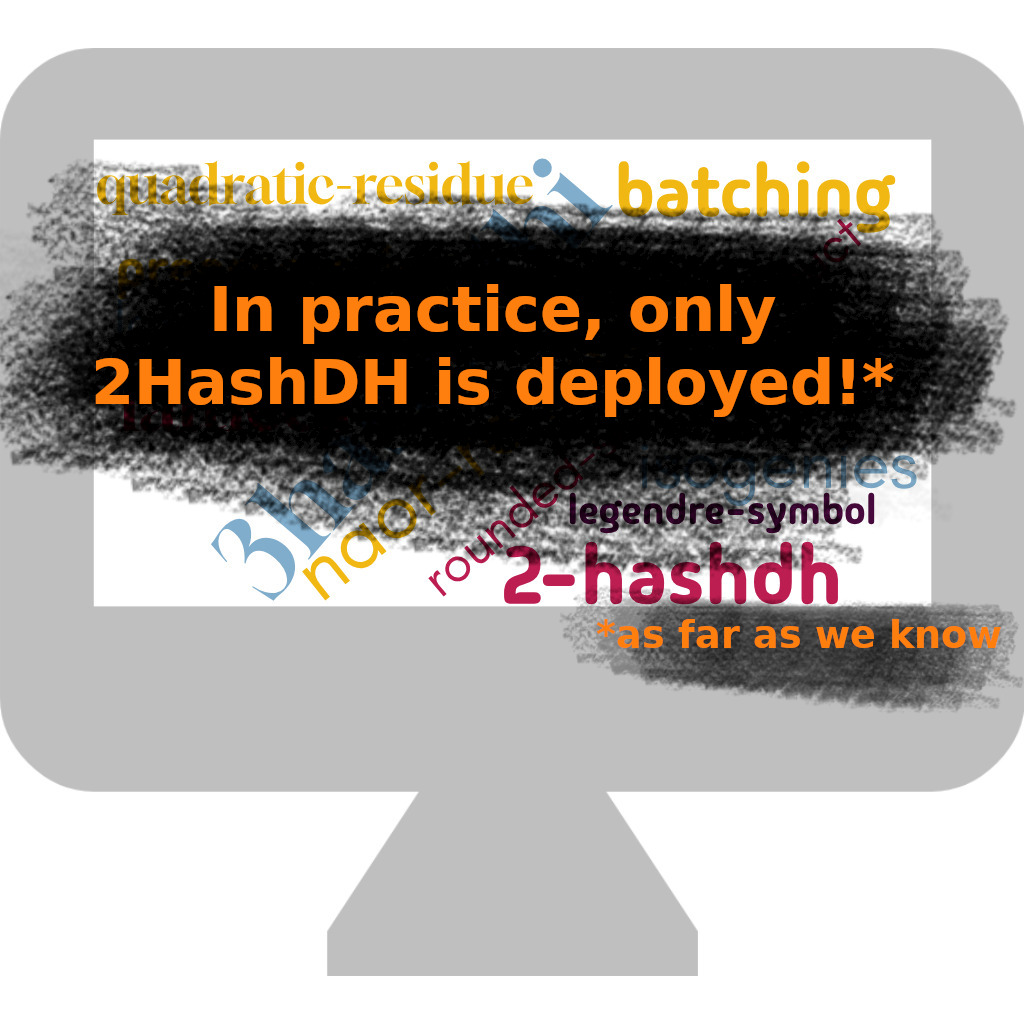
\includegraphics{figures/wordcloud-oprfs-2.jpg}
\end{frame}

\begin{frame}
  \frametitle{RFC 9497 at IETF~\cite{rfc9497}}
  \begin{itemize}
    \item OPRFs presented at NIST’s 2023 Multi-party Threshold Scheme workshop\pause
    \item IETF: only completed OPRF standard\pause
  \end{itemize}
  \begin{description}
    \item[OPRF] 2HashDH\pause
    \item[VOPRF] OPRF + $\pi(F_k(x),k)$\pause
    \item[POPRF] 
      Partial OPRF, the client submits a tag $t$ in addition to the
      input $x$ and gets the evaluation $y
      \coloneqq F_k (t, x)$. $t$ contains  additional information,
      e.g. a validity period.
  \end{description}
\end{frame}

\begin{frame}
  \frametitle{Could I use a blind signature instead of a VOPRF?}
  \begin{table}
    \begin{tabular}{l l r r}
      \toprule
      Protocol phase & action & blind RSA & VOPRF \\
      \midrule
      \multirow[c]{6}{*}{Issuance} & \multirow[c]{2}{*}{Client Blind} & 63 $\mu$s
                                   & 54 $\mu$s\\
                                   & & 256 bytes &  32 bytes \\
                                   & \multirow[c]{2}{*}{Server Evaluate} & 2.69 ms
                                   & 260 $\mu$s \\
                                   & & 256 bytes &  96 bytes \\
                                   & \multirow[c]{2}{*}{Client Finalize} & 37
                                   $\mu$s
                                   & 376 $\mu$s \\
                                   & & 256 bytes &  64 bytes \\
                                   \midrule
      \multirow[c]{4}{*}{Redemption} & \multirow[c]{2}{*}{Client} & -
                                     & -\\
                                     & & 300 bytes &  96 bytes \\
                                     & \multirow[c]{2}{*}{Server} & 37 $\mu$s
                                     & 57 $\mu$s \\
                                     & & - &  - \\
                                     \bottomrule
    \end{tabular}
    \caption{Comparing runtimes between blind signatures and VOPRFs,
    Source: \url{https://blog.cloudflare.com/private-rate-limiting/\#how-much-does-this-all-cost}}
  \end{table}\pause
  \alert{Also, OPRFs are amortizable!}
\end{frame}

\begin{frame}
  \frametitle{Overview of deployed primitives}
  \begin{table}
    \small
    \centering
    \begin{tabular}{ccc}
      \toprule
      Category & Name & Application type \\
      \midrule
                                                    \multirow[c]{1}{*}{unlinkability}  
               & CAPTCHAs & rate limiting         \\
                                                    & Kagi & unlinkable search         \\
                                                    & MoQ 
                                                    & authentication \\
                                                    \midrule
                                                    \multirow[c]{1}{*}{ protect low-entropy secrets}  
                                                    & Whatsapp  & authentication \\
                                                    \midrule
                                                    \multirow[c]{4}{*}{PSI}  
                                                    &  Google CCC & set intersect. \\
                                                    &  Microsoft CCC & set intersect. \\
                                                    &  MIGP & set intersect. \\
                                                    &  Ad-to-purchase & set intersect. \\
                                                    \midrule
                                                    \multirow[c]{4}{*}{deterministic identifiers}  
                                                    & Callisto & matching   \\
                                                    &  human.world & identifier \\
                                                    &  TACEO:OPRF & identity  \\
                                                    &  MetaMask & identity \\
                                                    \bottomrule
    \end{tabular}
    \label{tab:categories}
  \end{table}
\end{frame}


\section{Getting Unlinkability}

\begin{frame}
  \frametitle{Application: PrivacyPass}
  %  \resizebox{\textwidth}{!}{
  \procedureblock[mode=text]{}{%
    \qquad \textbf{Client} \> \> \textbf{Server} \((k)\)\\
    \textbf{1. Gather:} \> \>\\
    \qquad Choose \({\{x_{1},\ldots,x_{30}\}}\) \> \sendmessagerightleft*[14em]{OPRF}\>\\
    %\sendmessagerightleft*[16em]{\text{Issue Tokens}} \> \\
    \qquad Receive \({\{F_{k}(x_i)\}}_{ \in [30]}\) \> \>\\
    \textbf{2. Redeem:}  \> \>\\
    \>\sendmessageright*[14em]{x_i, F_{k}(x_i)} \>
  }
  %  }
\end{frame}

% \begin{frame}{Application: PrivacyPass}
% 
% \begin{procedureblock}{}
% \textbf{Client} \> \> \textbf{Server} $(k)$ \\
% \addlinespace[0.4em]
% \textbf{Phase 1: Gather} \\
% \> Choose $x_1,\dots,x_{30} \in \mathcal{X}$ \\
% \> \sendmessageright*{$x_1,\dots,x_{30}$} \\
% \> \sendmessageleft*{$F_k(x_1),\dots,F_k(x_{30})$} \\
% \addlinespace[0.6em]
% \textbf{Phase 2: Redeem} \\
% \> \sendmessageright*{$x_i,\; F_k(x_i)$}
% 
% \end{procedureblock}
% 
% \end{frame}
% 

\begin{frame}{Applications}
  \begin{itemize}
    \item Reduces number of CAPTCHAs by factor
      30~\cite{ietf-privacypass-protocol-04}
    \item Authentication for Media over
      Quic~(MoQ)~\cite{ietf-moq-privacy-pass-auth-01}  
    \item Kagi~\cite{kagi}: anonymous identity for unlinkable search
  \end{itemize}
  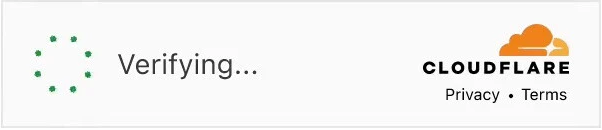
\includegraphics[scale=0.4]{figures/robot-checkbox.png}
\end{frame}

\section{Deterministic high-entropy output from low-entropy secrets}

\begin{frame}{Private Set Intersection~(PSI)}
  OPRFs are useful for \alert{unbalanced} sets, where one party, typically the
  server in client-server protocols, has a significantly larger set than the
  other party.\pause
  \begin{figure}
    \centering
    \procedureblock[mode=text]{}{%
      \textbf{Client} \((x_{1}, \ldots, x_{m})\) \> \> \textbf{Server} \((y_1,
      \ldots, y_n), k\)\\
      \({\{F_{k}(x_i)\}}_{i \in [m]}\) \> \sendmessagerightleft*[16em]{VOPRF
      } \> \\
      \> \sendmessageleft*[16em]{\{z_j = F_k(y_i)\}_{j \in [n]}} \>\\
    }
    \(F_{k}(x_i) = z_{j}\).
    Otherwise \(F_{k}(y_j)\) is pseudorandom.
  \end{figure}\pause
  \hspace*{\fill} \alert{VOPRF: per-client keys may cause segmentation when
  output is revealed}
\end{frame}
\begin{frame}
  \frametitle{Applications using OPRFs for unbalanced set intersection}
  \begin{itemize}
    \item Google advertisement view to purchase conversion~\cite{EUROSP:IKNPSSRSY20} \pause
    \item Google~\cite{USENIX:TPYRKI19}/Microsoft CCC~\cite{microsoft-ccc}: check if credential appeared in breach\pause
    \item Cloudflare Might I Get Pwned~(MIGP)~\cite{ppccc-cloudflare}: checks if credential or
      \emph{related} credential have been leaked\pause
  \end{itemize}
  \alert{No schemes use verifiability. }\pause \\ 
  POPRFs are not useful. 
\end{frame}

\section{OPRFs for identitification: OPAQUE and identifiers}
\begin{frame}{OPAQUE: Authenticate without revealing password}
  \vspace{-3em}
  \procedureblock[mode=text]{}{%
    \qquad \textbf{Client} (pwd)  \> \> \textbf{Server} (k)\\
    \textbf{1. Registration:} \> \>\> \\
    \qquad \(k' = F_{k}(pwd)\) \>  \sendmessagerightleft*[16em]{OPRF} \> \\
    \qquad  Sample \((pk, sk)\) \> \sendmessageright*[16em]{pk, ct=Enc_{k'}(sk)} \> Store \((pk, ct)\)\\
    \uncover<2->{
      \textbf{2. Login:} \>\> \\ 
      \>\sendmessageleft*[16em]{ct} \>\\
      \qquad \(k' = F_{k}(pwd)\) \>\sendmessagerightleft*[16em]{OPRF} \> \\
      \qquad \(sk = Dec_{k'}(ct)\) \>\sendmessagerightleft*[16em]{\text{AKE using }sk} \>
    }
  }\pause
  \begin{itemize}
    \item IETF RFC 9807~\cite{rfc9807}\pause
    \item Whatsapp: avoid revealing backup PIN~\cite{whatsapp-whitepaper}
  \end{itemize}
\end{frame}


\begin{frame}
  \frametitle{Identites and Wallet keys from low-entropy outputs in a Threshold
  setting}
  \begin{description}
    \item[Threshold] A TOPRF enables a valid evaluation from a $m$-out-of-$n$ servers.\pause
  \end{description}
  \begin{itemize}
    \item Callisto~\cite{COMPASS:RQABLV18} to detect serial perpetrators of
      sexual misconduct while preserving victim privacy\pause
    \item identities from OPRF input: 
      \begin{itemize}
        \item MetaMask~\cite{metamask}
        \item TACEO OPRF~\cite{taceo-oprf}
        \item human.world~\cite{human}
      \end{itemize}\pause
    \item value
      \alert{MPC-friendliness!}
  \end{itemize}
\end{frame}

\section{MPC-friendly OPRFs}

\begin{frame}{Public Verifiability}
  Generate ZKP for evaluation with correct key.\\
  \pause Stronger and more flexible than VOPRF: 
  \begin{itemize}
    \item  anyone can verify ZKP tying input and
      evaluation together\pause
    \item can prove \emph{without} revealing input (dlog equivalent cannot do
      this)
      %  \item Composable: prove additional properties (e.g. within validity period,
      %    have certain passport and age $\geq$ 18)\pause
  \end{itemize}
  % TODO pic
\end{frame}

\begin{frame}{Optimizing for fewer constraints}
  \begin{itemize}
    \item 
      each constraint requires additional computation
    \item R1CS: each equality constraint has one multiplication and unlimited
      additions \\ \pause $\rightarrow$ use a cipher with low multiplicative depth\pause
    \item Example: commit to the challenge with Poseidon2 instead of SHA2
      \\ 2 orders of magnitude fewer constraints\pause
    \item BabyJubJub as a curve: 
      \begin{itemize}
        \item base field is the same as the scalar field as prove system\\ $\rightarrow$
          directly operate on the $(x,y)$
          coordinate representation
      \end{itemize}
  \end{itemize}
\end{frame}

% 
% \begin{frame}{Public Verifiability from R1CS}
%   \small
%   \begin{algorithmic}[1]
%     \Function{prove\_oprf}{$(y, \mathrm{com}, K), (x, \beta, r, e, s, B)$}
%     \State
%     \Comment{Public inputs: $(y, \mathrm{com}, K)$}
%     \State
%     \Comment{Private inputs: $(x, \beta, r, e, s, B)$}
%     \State $\mathrm{com}' \gets H_{\mathrm{com}}(x, r)$
%     \Comment{240 R1CS constraints (Poseidon2)}
%     \State \texttt{assert} $\mathrm{com}' = \mathrm{com}$
%     \State $Q \gets \mathsf{hash\_to\_curve}(x)$
%     \Comment{800 R1CS constraints}
%     \State $A \gets \beta \cdot Q$
%     \Comment{2300 R1CS constraints}
%     \State \texttt{assert} $\texttt{DLogEQ.Verify}(A, G, B, K, (e, s))$
%     \Comment{12000 R1CS constraints}
%     \State $Q_2 \gets \beta^{-1} \cdot B$
%     \Comment{2300 R1CS constraints}
%     \State $y' \gets H_2(x, Q_2)$
%     \Comment{2600 R1CS constraints}
%     \State \texttt{assert} $y' = y$
%     \EndFunction
%   \end{algorithmic}
% 
%   \vspace{0.5em}
%   \alert{\textbf{Complexity:} 20240 R1CS constraints (Comparison: SHA256 has
%     27734 constraints!)\pause
%     \begin{itemize}
%       \item[$\approx$] 1 ms VOPRF
%       \item[$\approx$] $<$ 3 ms with $t=3$
%   \end{itemize}}
% \end{frame}
\begin{frame}{Public Verifiability from R1CS}
  \vspace{5em}
  \begin{itemize}
    \item 20240 R1CS constraints to prove OPRF with Poseidon2 and BabyJubJub
    \item Comparison: SHA256 has
      27734 constraints!)\pause
    \item $\approx$ 1 ms VOPRF \pause
    \item $\approx$ $<$ 3 ms with $t=3$\pause
  \end{itemize}
  \hfill
  \only<1->{
    \begin{columns}
      \begin{column}{0.3\textwidth}
        \hfill
        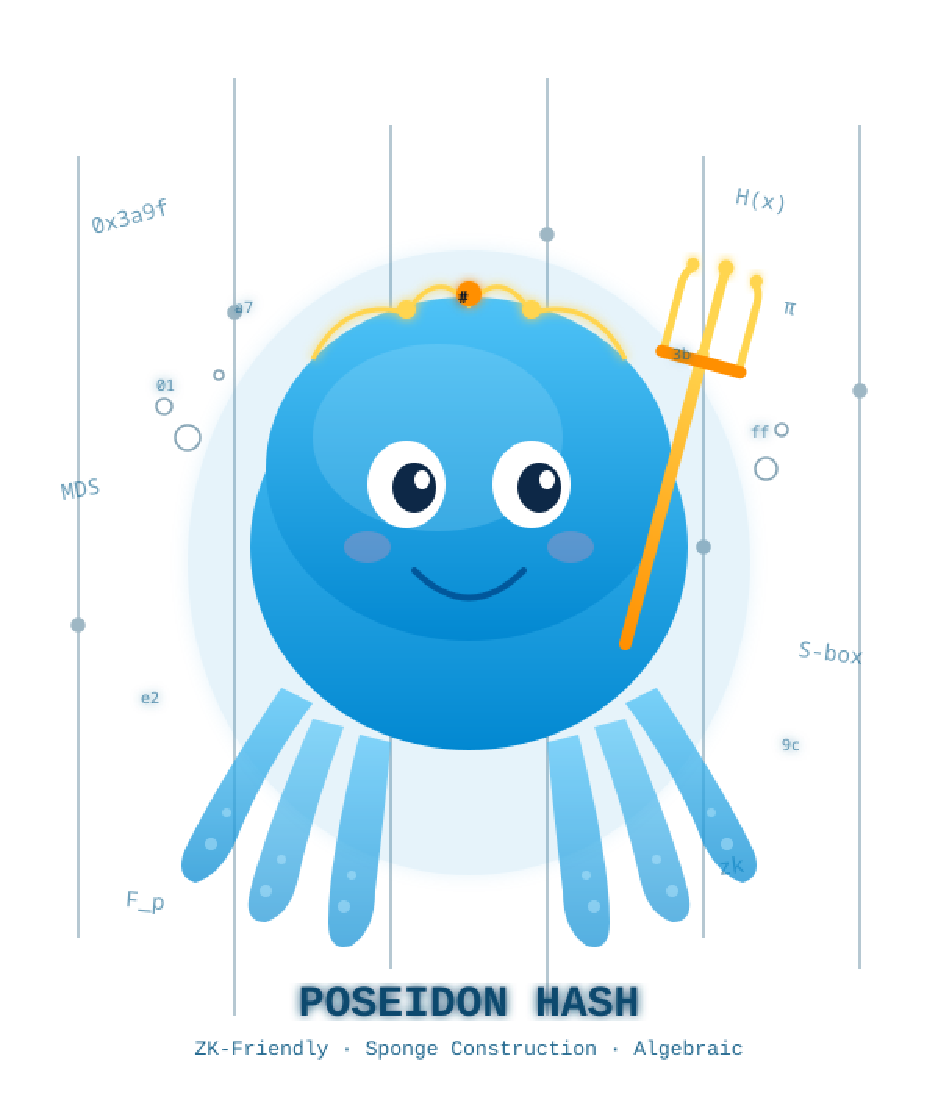
\includegraphics[scale=0.2]{figures/poseidon_svg-tex.pdf}
      \end{column}
      \begin{column}{0.49\textwidth}
        \hfill
\includegraphics[scale=0.2]{figures/baby-jub-jub.png}
      \end{column}
  \end{columns}}
\end{frame}

\begin{frame}{Recursive Verification}
  \begin{itemize}
    \item Trivial threshold setting: verify $m$ proofs per OPRF \pause
    \item Recursive Verification: threshold verification can be aggregated into
      a single proof\pause
    \item 
      responses are gathered by an accumulator\pause
    \item 
      2 challenge/response interactions
    \item 
      no communication between the servers\pause
  \end{itemize}
  \alert{More expensive to generate proof, easier verification!}
\end{frame}
% \begin{frame}{Public Verifiability from Schnorr}
%   \begin{itemize}
%     \item Stronger than verifiability: zero-knowledge proof tying input and
%       correct evaluation together
%     \item can prove \emph{without} revealing input (dlog equivalent cannot do
%       this)
%     \item Composable: prove additional properties (eg.g. within validity period,
%       have an Austrian passport and age is above 18)
%   \end{itemize}
% \end{frame}


\begin{frame}
  \begin{table}[htbp]
    \setlength{\tabcolsep}{4pt}
    \centering
    \caption{\small Compute cost microbenchmarks from TACEO deployment: query(\textbf{Q.}),
      answer (\textbf{A.}) and finalization (\textbf{Fin.}), as well as overall communication
      complexity(\textbf{comm.}).
    Publicly verifiable Groth16 proof is given in the \textbf{Prov.} column.}
    \label{tab:oprf_bench}
    \resizebox{\textwidth}{!}{
      \begin{tabular}{l c c c c c c c}
        \toprule
        \textbf{Setting} & \textbf{Client Q.} & \textbf{Server A.} & \textbf{Client Fin.} & \textbf{Rounds} &  \textbf{Server Comm.} & \textbf{Client Comm.} &\textbf{Prov.} \\
                         & \multicolumn{1}{c}{[$\mu s$]} & \multicolumn{1}{c}{[$\mu s$]} & \multicolumn{1}{c}{[$\mu s$]} &  & \multicolumn{1}{c}{[bytes]}  & \multicolumn{1}{c}{[bytes]}  & \multicolumn{1}{c}{ [$ms$]}\\
                         \midrule
        Single-server OPRF         & $128$ & $90$  & $99$    & 2 & 32& 32 &  - \\
        Single-server VOPRF        & $128$ & $468$ & $974$   & 2 & 32& 96 & $32$ \\
        \midrule
        TOPRF ($t=3$)     & $128$ & $90$  & $105$   & 2 & 32 & 32 & - \\
        TOPRF ($t=5$)     & $128$ & $468$ & $105$   & 2 & 32 & 32 & - \\
        TOPRF ($t=30$)    & $128$ & $468$ & $108$   & 2 & 32 & 32 & - \\
        TVOPRF ($t=3$)    & $128$ & $90$  & $2730$  & 2 & 32 & 96 & $55$ \\
        TVOPRF ($t=5$)    & $128$ & $468$ & $4480$  & 2 & 32 & 96 & $97$ \\
        TVOPRF ($t=30$)   & $128$ & $468$ & $26358$ & 2 & 32 & 96 & $712$\\
        \midrule
        Public TVOPRF (all $t$) & $147$ & $653$ & $1175$ & 4 &  192& 192 & $32$ \\
        \bottomrule
      \end{tabular}
    }
  \end{table}

\end{frame}


\begin{frame}
  \frametitle{Conclusion}
  \begin{itemize}
    \item wide applications for lightweight primitives
    \item extensions give rise to a number of protocols
    \item MPC+ZK gives efficient OPRFs: 
      \begin{itemize}
        \item use zk-friendly curves
        \item use zk-friendly hash functions
        \item \alert{constant} verification cost for the client 
      \end{itemize}
  \end{itemize}

\end{frame}

\begin{frame}
  \frametitle{Thank you!}

  \begin{table}
    \centering
    \resizebox{\textwidth}{!}{
      \begin{tabular}{cccccccc}
        Name & Application type & no reused $x$ & used curve & VOPRF & POPRF & TOPRF
        \\ \hline
        CAPTCHAs  & rate limiting & \faCheck & \shortstack{\faMugHot, \faCoffee,P-256,\\
        P-384, P-512}& \faCheck & \faCheck & \faTimes%  & \cite{rfc9497}
        \\
        MoQ                                             & authentication & \faCheck & \shortstack{\faMugHot, \faCoffee,P-256,\\
      P-384, P-512} & \faCheck & \faCheck & \faTimes\\
        Kagi & unlinkable search & \faCheck & \faMugHot & \faCheck & \faTimes & \faTimes
        \\
        Whatsapp  & authentication & \faTimes & ? & \faTimes & \faCheck & \faTimes \\
      Google CCC & set intersect. & \faTimes & \faLock' &  \faTimes & \faTimes & \faTimes \\
      Microsoft CCC & set intersect. & \faTimes & ? &  \faTimes & \faTimes & \faTimes \\
      MIGP & set intersect. & \faCheck$^\dagger$ & \faLock &  \faTimes
                                   & \faTimes & \faTimes\\
      Ad-to-purchase & set intersect. & \faTimes & ? & \faTimes & \faTimes & \faTimes\\
      Callisto
                    & matching & \faTimes  & P-384, \faMugHot &
      \faCheck & \faTimes & \faTimes%  & discontinued? &
      \\
      human.world & identifier &  \faTimes & \faBaby, \faLock & \faCheck &
      \faTimes &\faCheck \\
      TACEO:OPRF & identity  & \faCheck  & \faBaby &
      \faCheck$^{\ddagger}$ & \faTimes & \faCheck \\
      MetaMask & login & \faTimes & P-256, P-384 & \faCheck & \faTimes & \faCheck\\
      %    Email set intersection & email intersection & \faTimes & &  & % cloudflare/voprf-ts
    \end{tabular}
  }
  \caption{Protocols using OPRFs in practice. All implementations use the 2HashDH OPRF construction. $^\dagger$ Input $x$ is not repeated, but related. $^\ddagger$ Threshold proofs are aggregable into a single constant-size proof with efficient verification. \faMugHot~Ristretto255, \faCoffee~Decaf488, \faBaby~BabyJubJub,
  \faLock~Sekp256k1, \faLock'~Sekp224r1. }

  % TODO add user numbers
  \label{tab:applications}
\end{table}

\end{frame}

\begin{frame}[t]
  \frametitle{What about PQ?}
  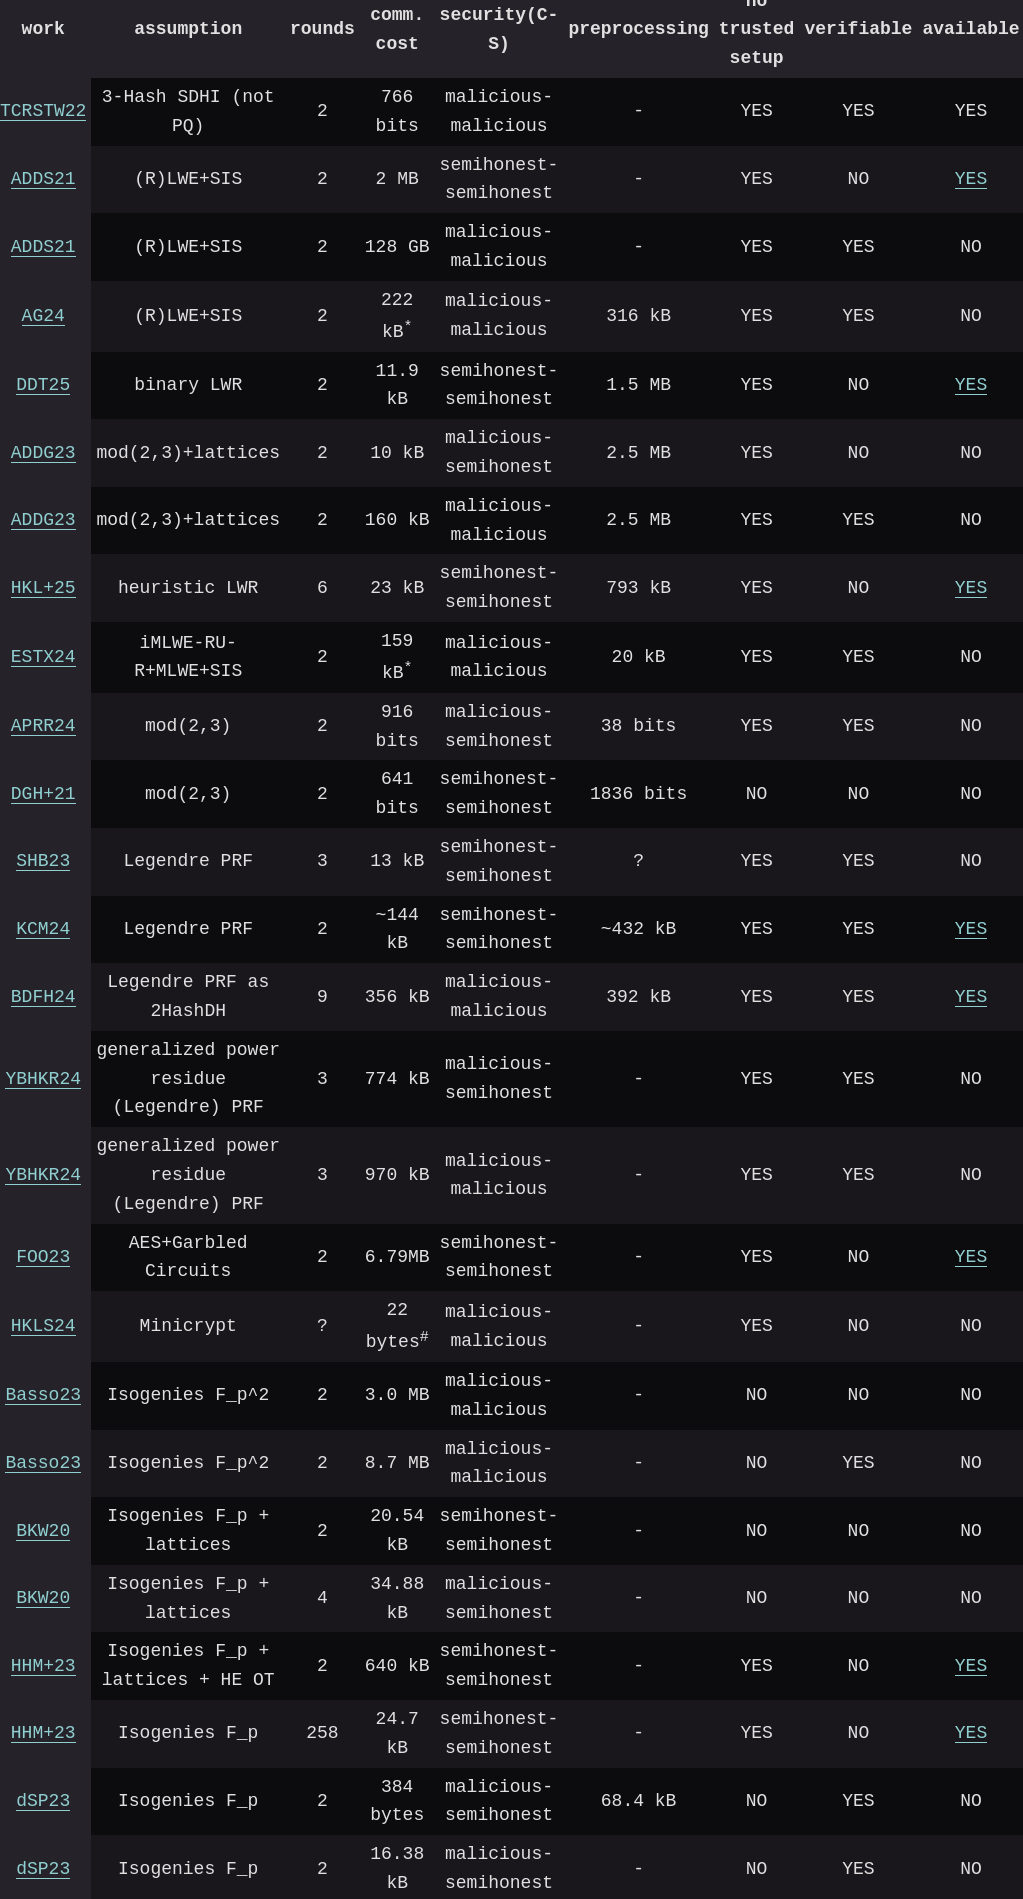
\includegraphics[scale=0.2]{figures/oprfs.png}
\end{frame}


\begin{frame}[allowframebreaks]
  \frametitle{References}

  \bibliography{bilbio,export/crypto,export/abbrev3}
  \bibliographystyle{alpha}

\end{frame}
\end{document}
